\documentclass[9pt]{beamer}
\usepackage{pdfpages}
\usepackage{caption}
\usepackage{fixltx2e}
% \usepackage{colortbl}
% \usepackage{subcaption}
\usepackage{slashed}
\usepackage{tikz}
\DeclareGraphicsExtensions{.pdf,.png,.jpg}

\usetheme{Luebeck}
\definecolor{cern}{RGB}{0,83,161}
 \setbeamercolor*{palette primary}{use=structure,fg=white,bg=cern}
\setlength{\parskip}{2.5mm}
\setbeamercolor{block title}{bg=cern}
\newenvironment{terminalblock}[1]{%
  \setbeamercolor{block body}{bg=black, fg=white}
  \begin{block}{#1}}{\end{block}}

\title[Beamline for Schools\hspace{2em}\insertframenumber/
\inserttotalframenumber]{Beamline for Schools\\DAQ and shift responsibilities}
\author{\emph{Tim Brooks}}
\institute{CERN / RHUL}
\date{2015-09-12}

\begin{document}
\setbeamertemplate{caption}{\centering\insertcaption\par}

\begin{frame}
\titlepage{}
\centering

\includegraphics[scale=0.1]{img/LogoBadge}
\,

\includegraphics[scale=0.049]{img/RHUL}
\end{frame}


\begin{frame}{T9 facilities}
\begin{columns}
  \begin{column}{.4\textwidth}
    \vspace*{-0.5cm}
    \begin{figure}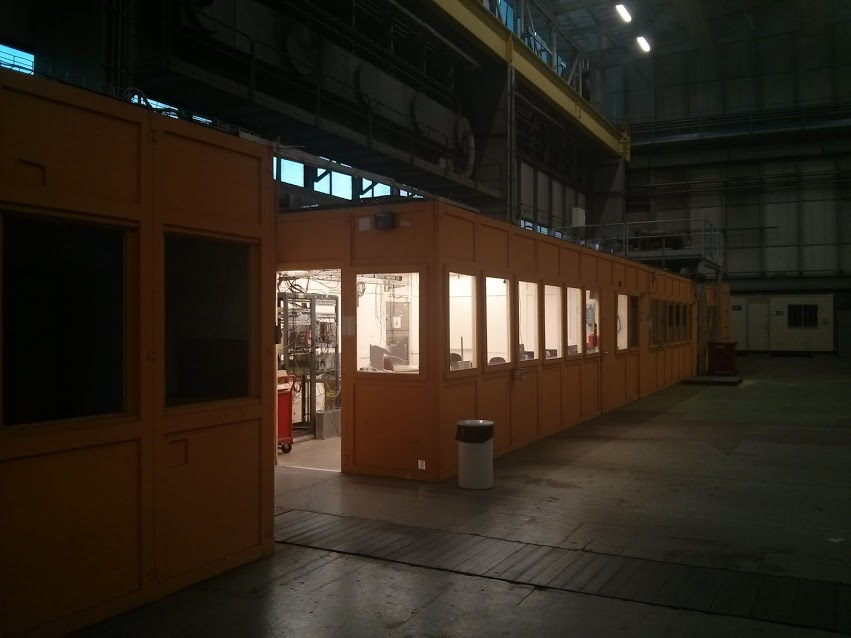
\includegraphics[scale=0.17]{img/Barrack}\vspace*{-0.2cm}\caption{T9 control room}\end{figure}\vspace*{-1cm}
  \end{column}
  \begin{column}{.4\textwidth}
    \vspace*{-0.5cm}
    \begin{figure}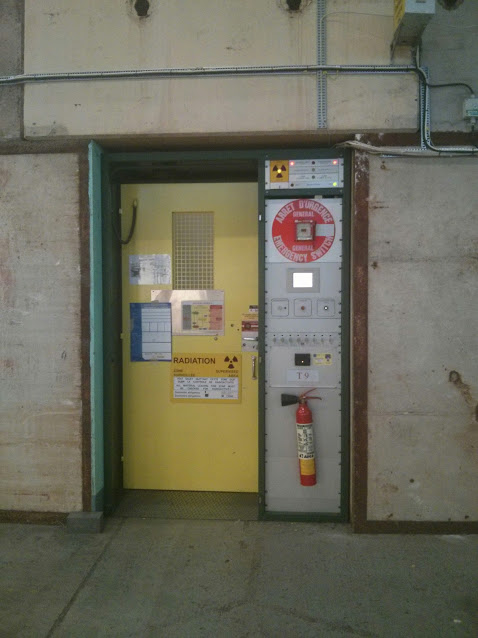
\includegraphics[scale=0.17]{img/PAD}\vspace*{-0.2cm}\caption{T9 experiment zone access door}\end{figure}\vspace*{-1cm}
  \end{column}
\end{columns}
\end{frame}

\begin{frame}{Experiment set-up}
\begin{figure}\centering
    % 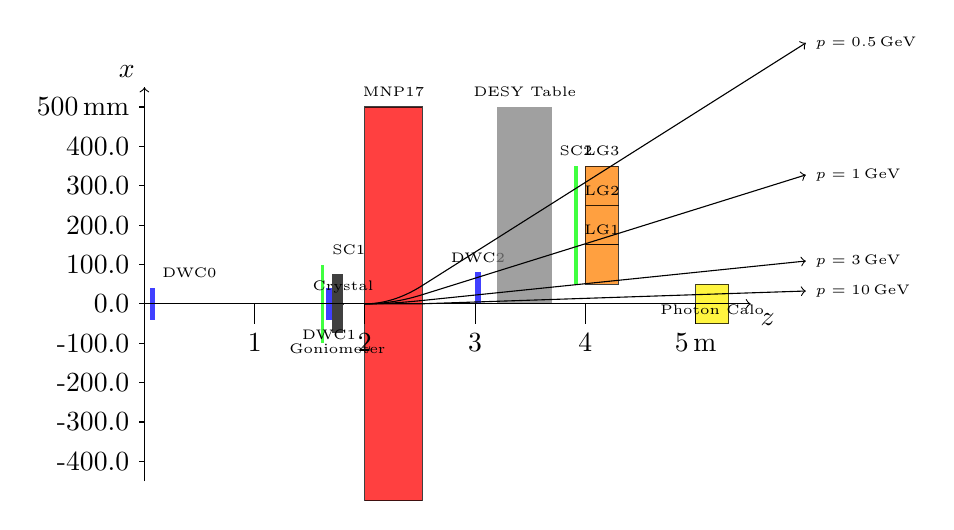
\begin{tikzpicture}[xscale=1.4,yscale=5]

\tikzset{add reference/.style={insert path={%
    coordinate [pos=0,xshift=-0.5\pgflinewidth,yshift=-0.5\pgflinewidth] (#1 south west)
    coordinate [pos=1,xshift=0.5\pgflinewidth,yshift=0.5\pgflinewidth]   (#1 north east)
    coordinate [pos=.5] (#1 center)
    (#1 south west |- #1 north east)     coordinate (#1 north west)
    (#1 center     |- #1 north east)     coordinate (#1 north)
    (#1 center     |- #1 south west)     coordinate (#1 south)
    (#1 south west -| #1 north east)     coordinate (#1 south east)
    (#1 center     -| #1 south west)     coordinate (#1 west)
    (#1 center     -| #1 north east)     coordinate (#1 east)
}}}

\coordinate (ref) at (0,0);
\coordinate (backref) at (-7.5,0);

%% Magnet
\fill[draw=black,fill=red,opacity=0.75,label=north:MNP18] (2,-0.5) rectangle ++(0.52, 1) [add reference=mnp17];
\node[anchor=south] at (mnp17 north) {\tiny{MNP17}};

%% Cherenkov
% \fill[draw=black,fill=gray,opacity=0.75] (-2.5,-0.1) rectangle ++(-5, 0.2) [add reference=ch0];
% \node[anchor=south] at (ch0 north) {\tiny{CH0}};

% \fill[draw=black,fill=gray,opacity=0.75] (0,-0.1) rectangle ++(-2.5, 0.2) [add reference=ch1];
% \node[anchor=south] at (ch1 north) {\tiny{CH1}};

%% Scint
% \fill[color=green,opacity=0.75] (0,-0.10) rectangle ++(0.03, 0.2) [add reference=sc0];
% \node[anchor=south west] at (sc0 north) {\tiny{SC0}};

\fill[color=green,opacity=0.75] (1.60,-0.10) rectangle ++(0.03, 0.2) [add reference=sc1];
\node[anchor=south west] at (sc1 north) {\tiny{SC1}};

\fill[color=green,opacity=0.75] (3.9,0.05) rectangle ++(0.03, 0.3) [add reference=sc2];
\node[anchor=south] at (sc2 north) {\tiny{SC2}};

%% DWC
\fill[color=blue,opacity=0.75] (0.05,-0.04) rectangle ++(0.05, 0.08) [add reference=dwc0];
\node[anchor=south west] at (dwc0 north) {\tiny{DWC0}};

\fill[color=blue,opacity=0.75] (1.65,-0.04) rectangle ++(0.05, 0.08) [add reference=dwc1];
\node[anchor=north] at (dwc1 south) {\tiny{DWC1}};

\fill[color=blue,opacity=0.75] (3,0) rectangle ++(0.05, 0.08) [add reference=dwc2];
\node[anchor=south] at (dwc2 north) {\tiny{DWC2}};

%% Calo
\fill[draw=black,fill=yellow,opacity=0.75] (5,-0.05) rectangle ++(0.3, 0.1) [add reference=photon_calo];
\node[anchor=south] at (photon_calo south) {\tiny{Photon Calo}};

\fill[draw=black,fill=orange,opacity=0.75] (4,0.25) rectangle ++(0.3, 0.1) [add reference=lg3];
\node[anchor=south] at (lg3 north) {\tiny{LG3}};

\fill[draw=black,fill=orange,opacity=0.75] (4,0.15) rectangle ++(0.3, 0.1) [add reference=lg2];
\node[anchor=south] at (lg2 north) {\tiny{LG2}};

\fill[draw=black,fill=orange,opacity=0.75] (4,0.05) rectangle ++(0.3, 0.1) [add reference=lg1];
\node[anchor=south] at (lg1 north) {\tiny{LG1}};

%% Crystal
\fill[color=black,opacity=0.75] (1.7,-0.075) rectangle ++(0.1, 0.15) [add reference=goniometer];
\node[anchor=north] at (goniometer south) {\tiny{Goniometer}};

\fill[color=black,opacity=0.75] (1.8,-0.002) rectangle ++(0.001, 0.004) [add reference=crystal];
\node[anchor=south] at (crystal north) {\tiny{Crystal}};

%% DESY table
\fill[color=gray,opacity=0.75] (3.2,0) rectangle ++(0.5, 0.5) [add reference=desytable];
\node[anchor=south] at (desytable north) {\tiny{DESY Table}};

%% Reference trajectories
% \draw[->] (mnp17 west) arc (-90:-89.4998:59.5650185) -- (5,0.0327) node[anchor=west] {\tiny{$p = 10\,\mathrm{GeV}$}};
\draw[->] (mnp17 west) -- (2.52,0.00027) -- (6,0.0327) node[anchor=west] {\tiny{$p = 10\,\mathrm{GeV}$}};
\draw[->] (mnp17 west) arc (-90:-88.3335:17.8695) -- (6,0.1089) node[anchor=west] {\tiny{$p = 3\,\mathrm{GeV}$}};
\draw[->] (mnp17 west) arc (-90:-84.992:5.9565) -- (6,0.3277) node[anchor=west] {\tiny{$p = 1\,\mathrm{GeV}$}};
% \draw[->] (mnp17 west)  arc  (-90:-91:595.7) node[anchor=west] {\tiny{$p = e\,\mathrm{GeV}$}};
\draw[->] (mnp17 west)  arc  (-90:-80:2.978) -- (6,0.6628) node[anchor=west] {\tiny{$p = 0.5\,\mathrm{GeV}$}};

% Draw main coordinate system
\draw[->] (ref) -- ++(5.5,0) node[anchor=north west]{$z$};
\draw (0,-0.45) -- (ref) -- ++(0,0.55);
% \draw (backref) -- (ref);
\draw[->] (0,-0.45) -- (ref) -- ++(0,0.55) node[anchor=south east]{$x$};

\foreach \x in {-4,-3,...,4}{
    \pgfmathsetmacro\result{\x * 100}
    \draw (0,0.1 * \x) -- ++(-0.05,0) node[anchor=east]{\result};
}
\draw (0,0.5) -- ++(-0.05,0) node[anchor=east]{500\,mm};

\foreach \z in {1,2,...,4}{
    \draw (\z,0) -- ++(0,-0.05) node[anchor=north]{\z};
}
\draw (5,0) -- ++(0,-0.05) node[anchor=north]{5\,m};

\end{tikzpicture}

    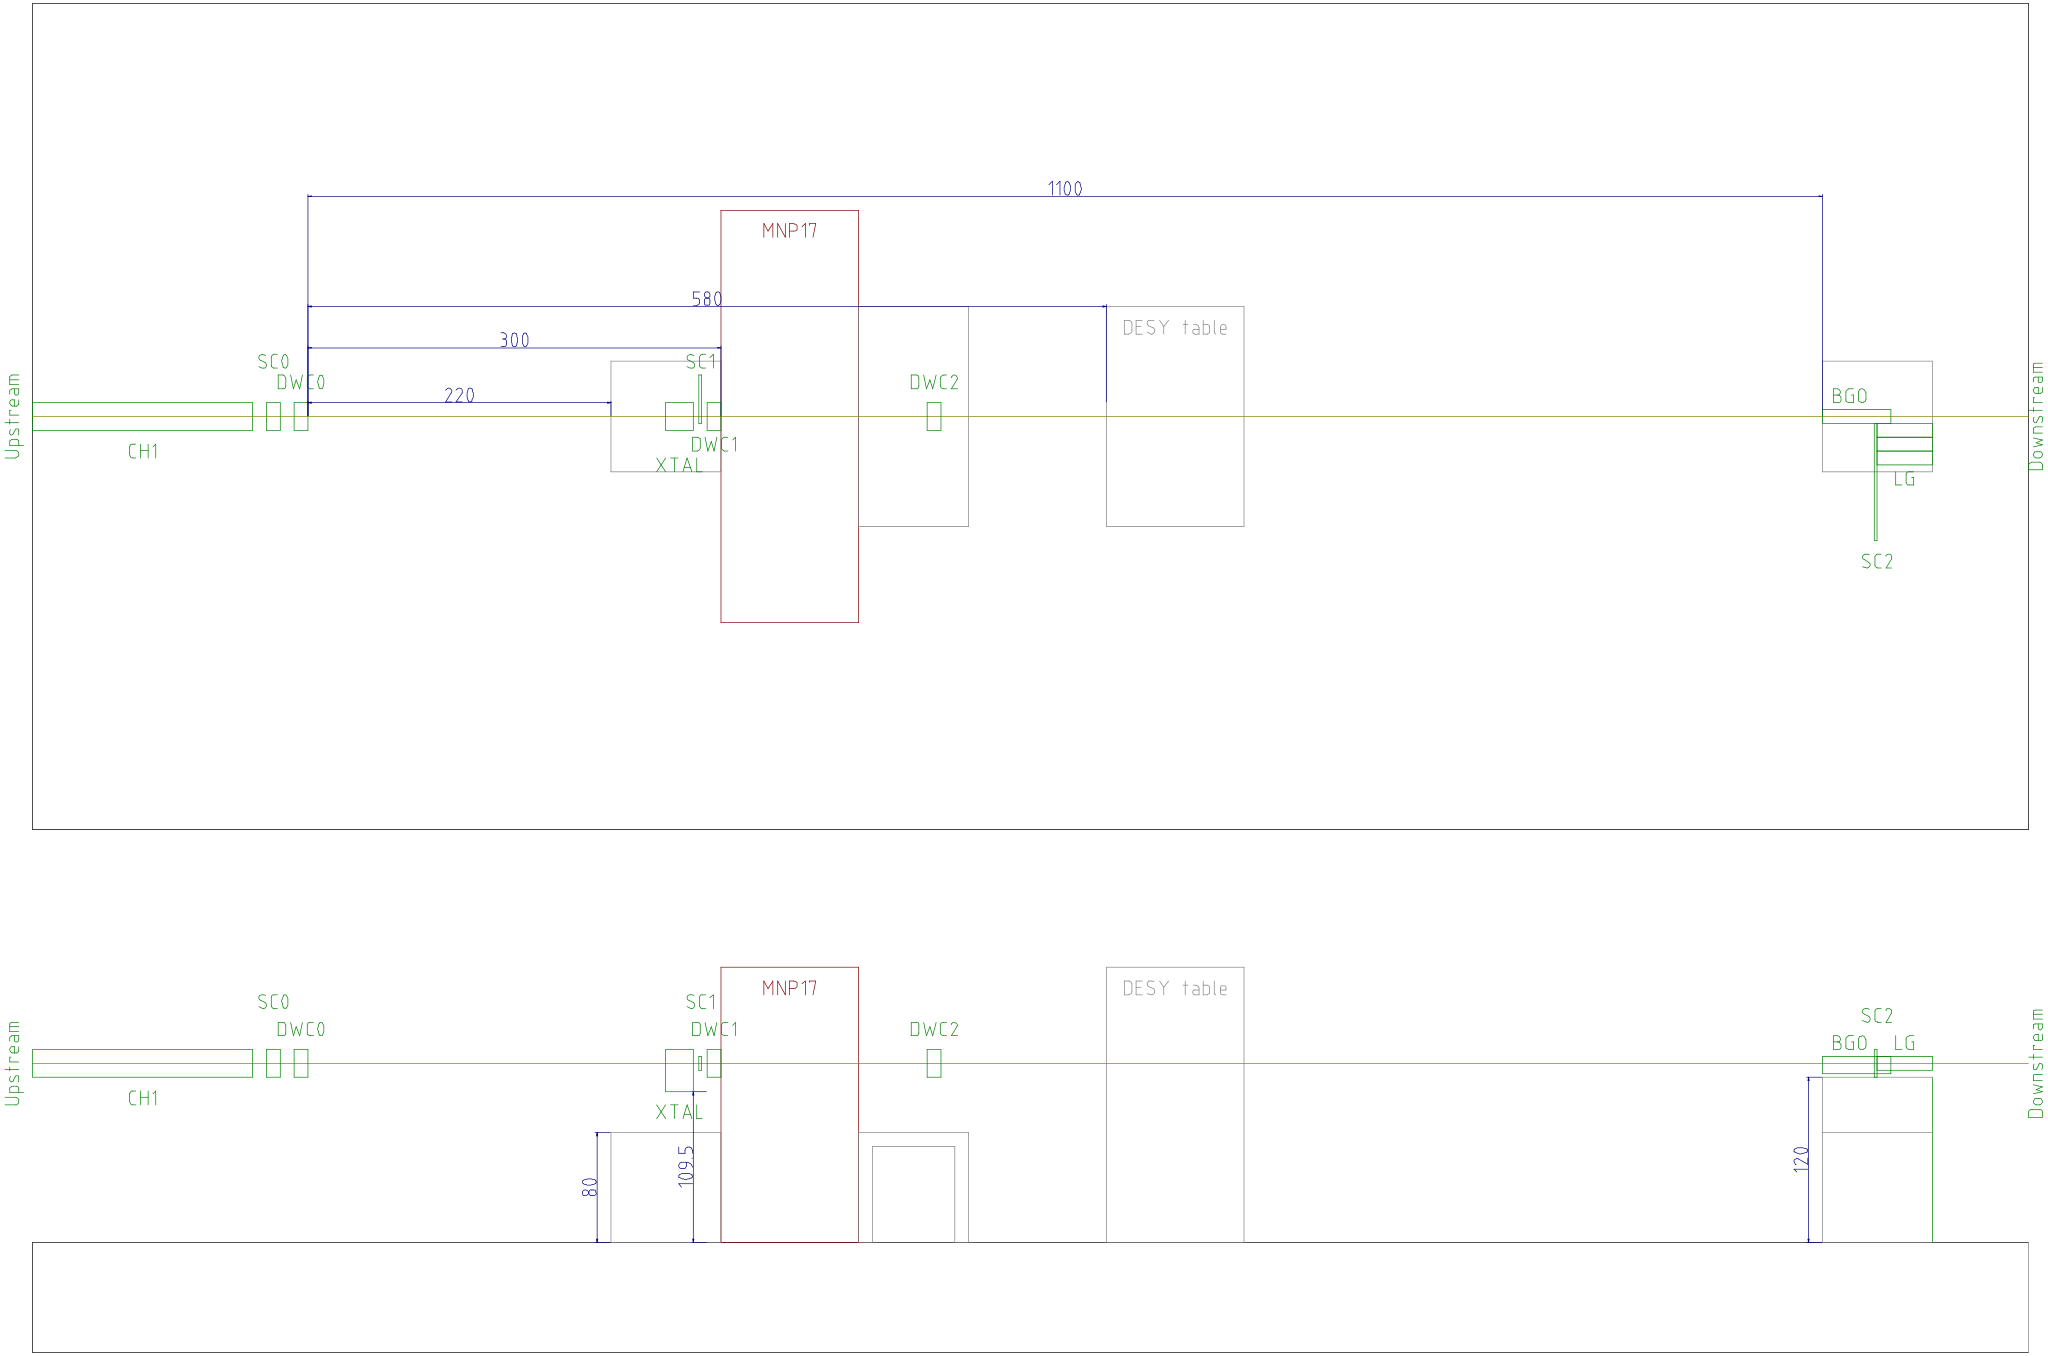
\includegraphics[scale=0.1]{img/t9_layout}
\end{figure}
\end{frame}

\section{Detectors}
\begin{frame}
\begin{center}
We {\tiny(ab)}use acronyms to refer to detector elements:

\begin{tabular}{|l|c|}\hline
    Detector type & Names \\\hline
    Cherenkov & CH0, CH1 \\
    Scintillator & SC0, SC1, SC2 \\
    Delay Wire Chamber & DWC0, DWC1, DWC2 \\
    Lead Glass Calorimeter & LG0, LG1, LG2, LG3 \\
    Bismuth Germanate Calorimeter & BGO \\
\hline
\end{tabular}
\end{center}
\end{frame}

\begin{frame}{PMT threshold detectors}
  \begin{columns}
    \begin{column}{.4\textwidth}
    \vspace*{-0.2cm}
    \begin{figure}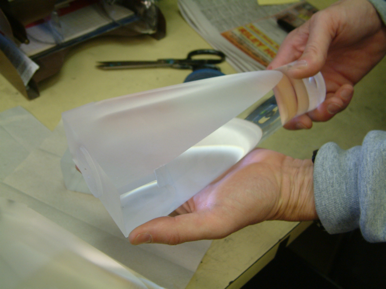
\includegraphics[scale=0.17]{img/Scint_plastic}\vspace*{-0.2cm}\caption{Scintillating plastic}\end{figure}\vspace*{-0.5cm}
    \begin{figure}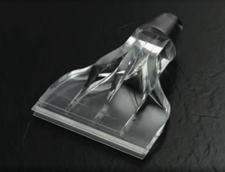
\includegraphics[scale=0.28]{img/Light_guide}\vspace*{-0.2cm}\caption{Light guide}\end{figure}\vspace*{-0.5cm}
    \begin{figure}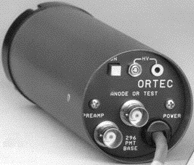
\includegraphics[scale=0.29]{img/PMT}\vspace*{-0.2cm}\caption{Photo-Multiplier Tube}\end{figure}\vspace*{-0.5cm}
    \end{column}
    \begin{column}{.6\textwidth}
    \vspace*{-0.5cm}
    \begin{figure}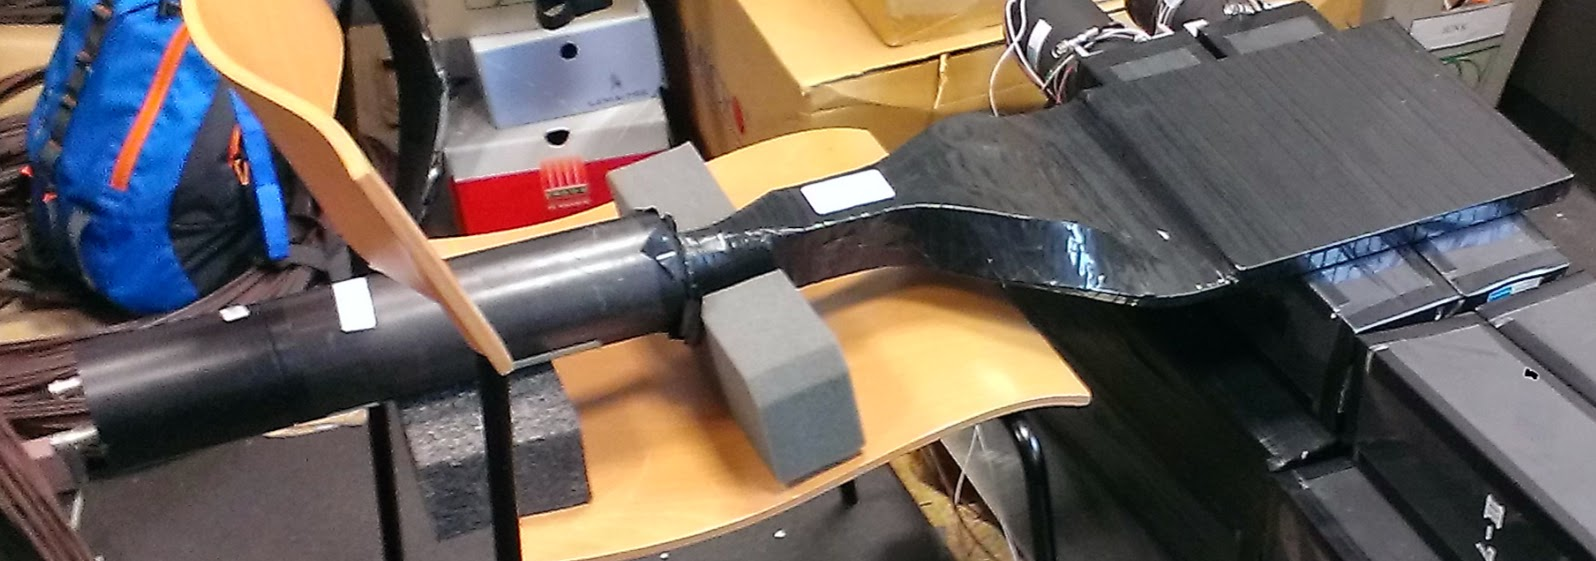
\includegraphics[scale=0.08]{img/Scintillator}\vspace*{-0.2cm}\caption{Scintillator assembly\newline- charged particle timing}\end{figure}\vspace*{-0.5cm}
    \begin{figure}\includegraphics[scale=0.03]{img/Cherenkov}\vspace*{-0.2cm}\caption{Cherenkov detector\newline- charged particle identification}\end{figure}\vspace*{-0.5cm}
    \end{column}
  \end{columns}
\end{frame}

\begin{frame}{PMT integral detectors}
  \begin{columns}
    \begin{column}{.4\textwidth}
      \begin{itemize}
        \item Absorb electromagnetic particles fully
        \item Energy converted to light
        \item PMT converts light into electrical pulse
        \item Integrate pulse to recover the particle energy
      \end{itemize}
    \end{column}
    \begin{column}{.6\textwidth}
    \vspace*{-0.5cm}
    \begin{figure}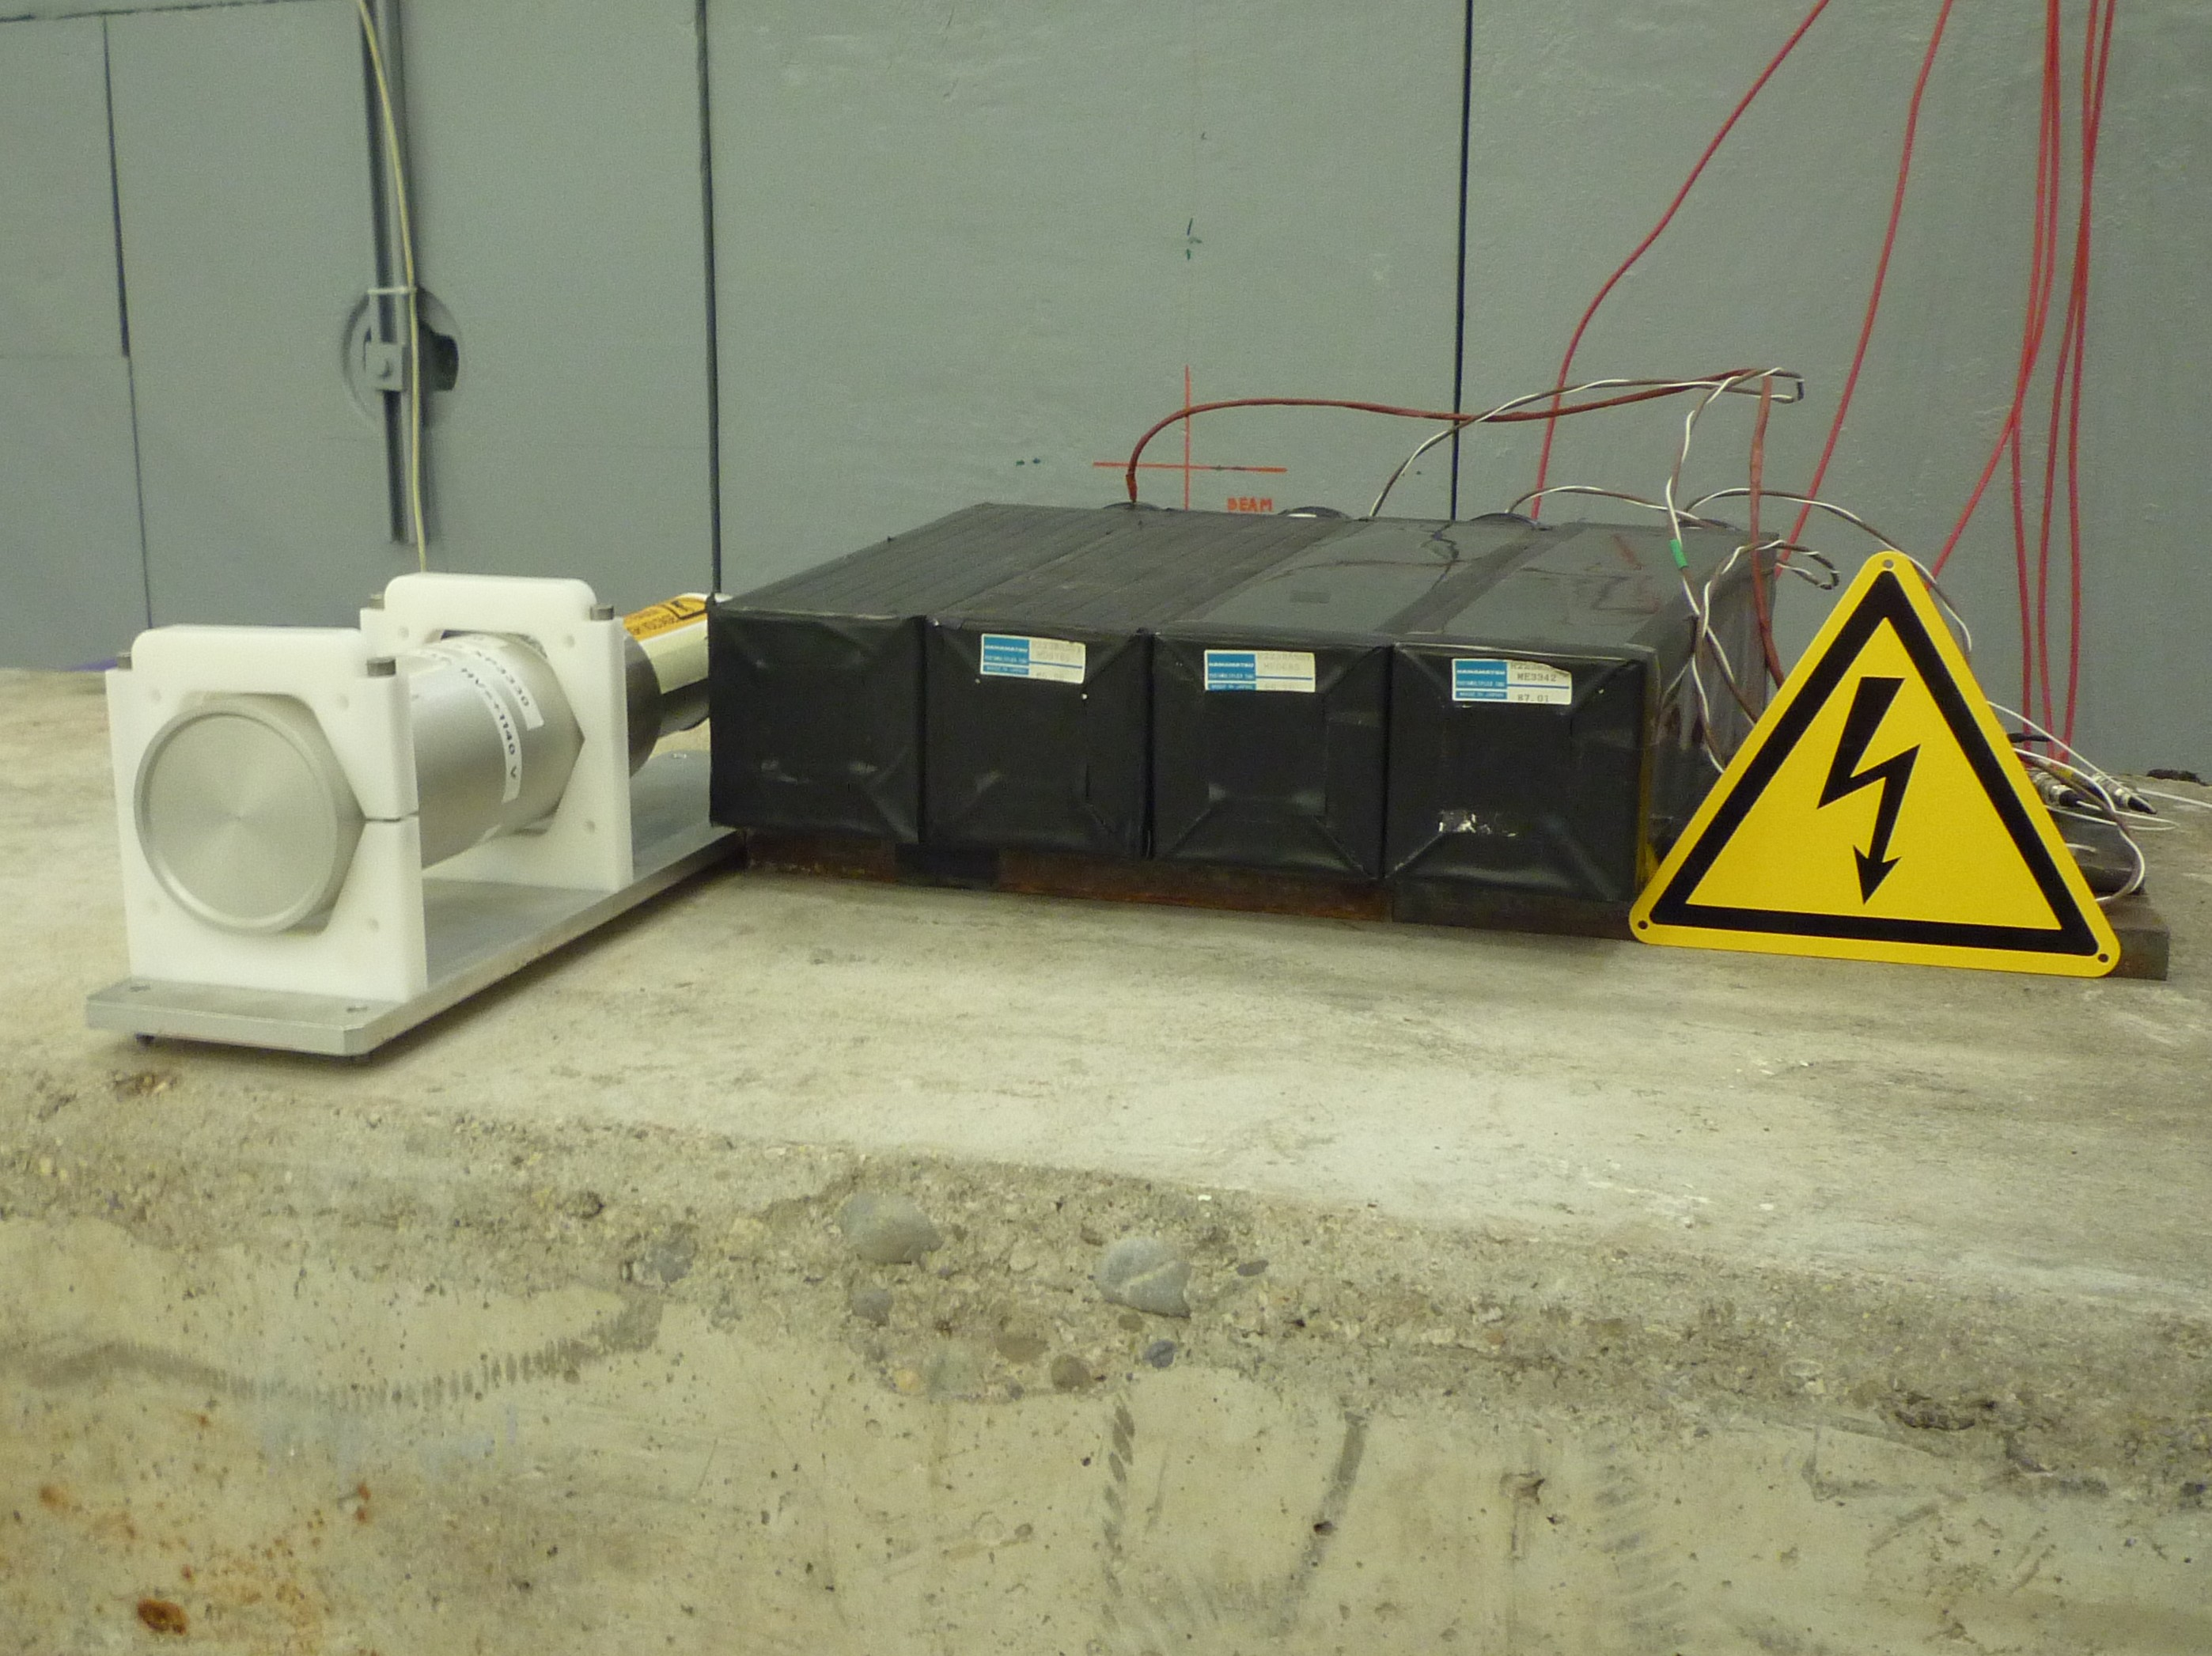
\includegraphics[scale=0.05]{img/Calo}\vspace*{-0.2cm}\caption{Calorimeter blocks}\end{figure}\vspace*{-1cm}
    \end{column}
  \end{columns}
\end{frame}

\begin{frame}{Delay wire chamber}
  \begin{columns}
    \begin{column}{.6\textwidth}
    \vspace*{-0.5cm}
    \begin{figure}\includegraphics[scale=0.05]{img/DWC}\vspace*{-0.2cm}\caption{Delay Wire Chamber (DWC0)}\end{figure}\vspace*{-1cm}
    \end{column}
    \begin{column}{.4\textwidth}
      \begin{itemize}
        \item Multi-Wire Proportional Chamber (MWPC)
        \item Charged particles ionise gas
        \item On board 'Front-end' electronics
        \item Two outputs per axis
        \item Compare the timing of signals on an axis
        \item Gives an X-Y location of hit
      \end{itemize}
    \end{column}
  \end{columns}
\end{frame}

\begin{frame}{Gas supply}
  \begin{columns}
    \begin{column}{.6\textwidth}
    % \vspace*{-0.5cm}
    The Delay Wire Chambers require gas to ionise
    \vspace{0.5cm}

    A supply of Argon and Carbon Dioxide (Ar + CO\textsubscript{2}) is provided from a distribution panel behind the beam control room
    \vspace{0.5cm}

    The Cherenkov detectors may be filled with Nitrogen or CO\textsubscript{2}
    \vspace{0.5cm}

    They can also be evacuated by vacuum pumps
    \end{column}
    \begin{column}{.4\textwidth}
    \vspace*{-0.5cm}
    \begin{figure}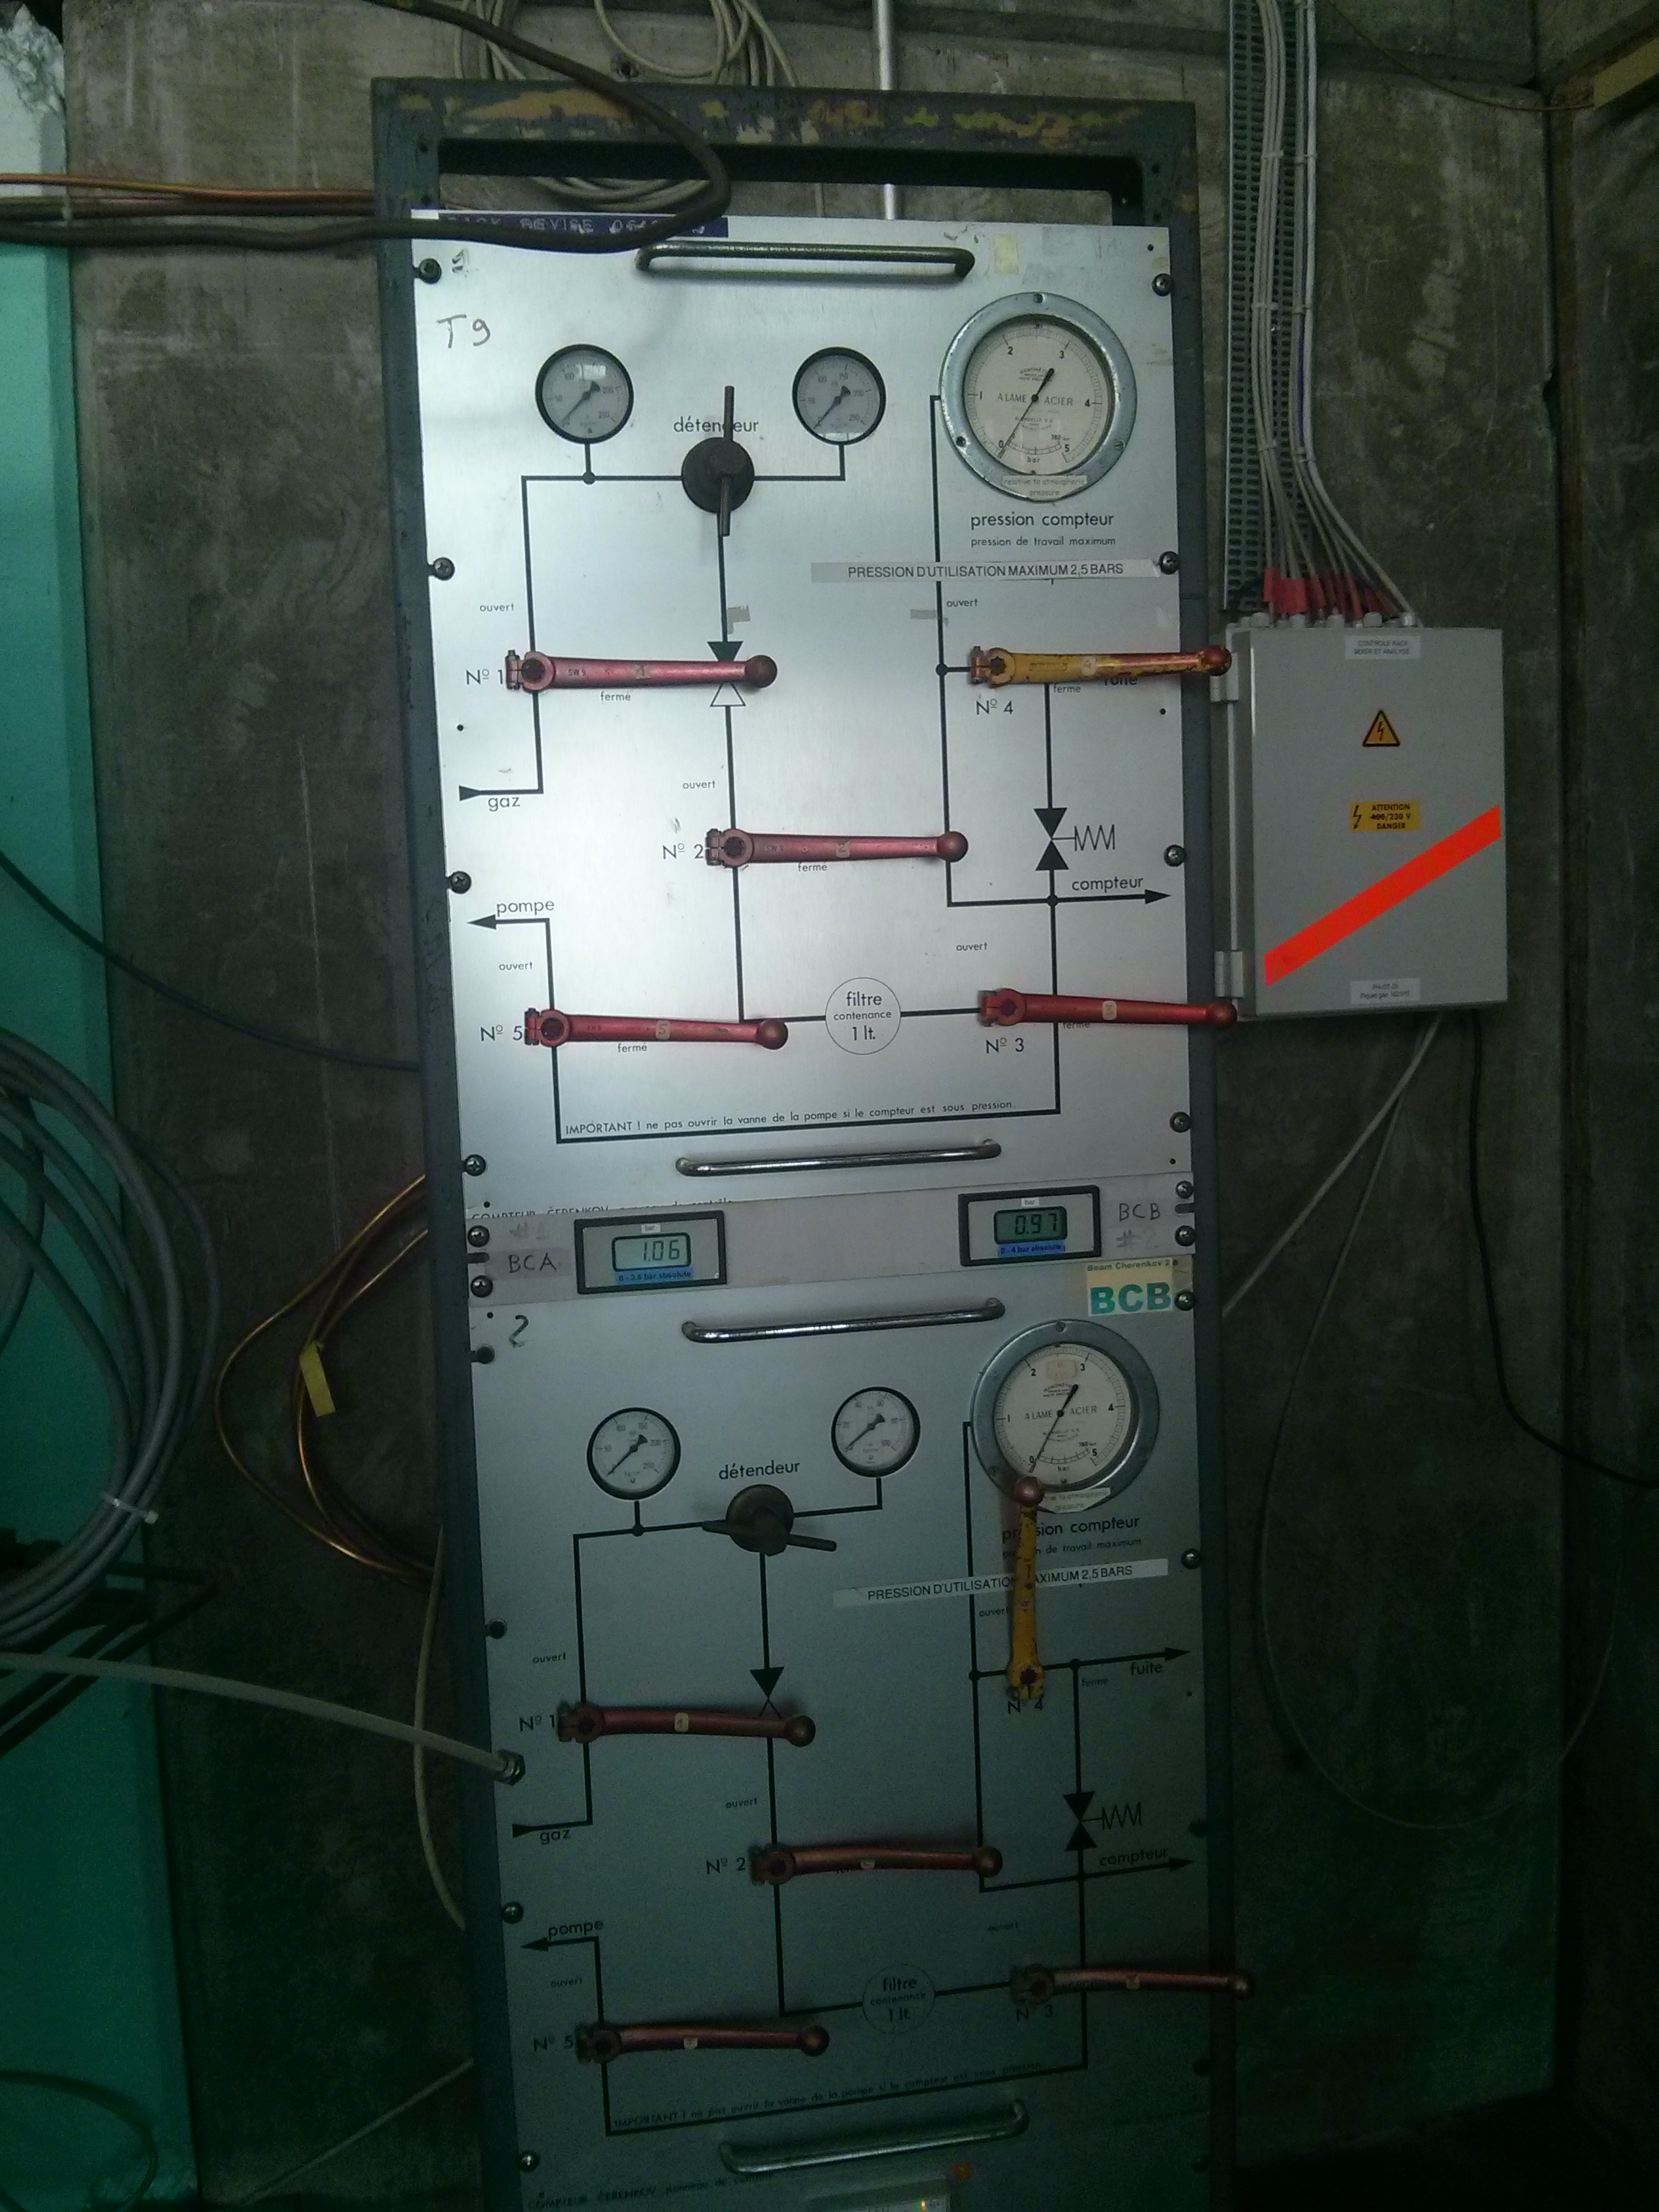
\includegraphics[scale=0.05]{img/Cherenkov_gas_control}\vspace*{-0.2cm}\caption{Cherenkov gas panel}\end{figure}\vspace*{-1cm}
    \end{column}
  \end{columns}
\end{frame}

\begin{frame}{Power supply}
  \begin{columns}
    \begin{column}{.6\textwidth}
    \vspace*{-0.5cm}
    \begin{figure}\includegraphics[scale=0.04]{img/HV}\vspace*{-0.2cm}\caption{HV crate and modules}\end{figure}\vspace*{-1cm}
    \end{column}
    \begin{column}{.4\textwidth}
    \vspace*{-0.5cm}
    \begin{itemize}
        \item Modular power supply unit
        \item Rack mount 'crate' holds modules, provides power and controls output
        \item Modules:
        \begin{itemize}
            \item A1833P 12 channels, $4\,\mathrm{kV}$ positive, $2\,\mathrm{mA}$
            \item A1833N negative voltage version of above
        \end{itemize}
        \item Modules monitor voltage and current usage, tripping off in case of problems
    \end{itemize}
        The Delay Wire Chamber also needs low voltage power from a bench top power supply
    \end{column}
  \end{columns}
\end{frame}

\section{Readout Electronics}
\begin{frame}{Analog electronics: NIM}
  \begin{columns}
    \begin{column}{.4\textwidth}
    \vspace*{-0.5cm}
    \begin{itemize}
        \item Nuclear Instrumentation Module (NIM)
        \item Modular standard for analog electronic components
        \item Rack mount 'bin' holds modules and provides power
        \item Modules:
        \begin{itemize}
            \item Amplifier
            \item Fan-in (logical OR), Fan-out
            \item Discriminator
            \item Coincidence\newline(logical AND)
            \item Timer
            \item Counter
        \end{itemize}
    \end{itemize}
    \end{column}
    \begin{column}{.6\textwidth}
    \vspace*{-0.5cm}
    \begin{figure}\includegraphics[scale=0.04]{img/NIM}\vspace*{-0.2cm}\caption{NIM bin and modules}\end{figure}\vspace*{-1cm}
    \end{column}
  \end{columns}
\end{frame}

\begin{frame}{Analog electronics: NIM}
  \begin{block}{Discriminator}
    A discriminator has two settings; a 'Threshold' and a 'Width'

    Noise with a voltage below the Threshold is ignored

    If the input signal crosses the Threshold, a pulse is generated with the desired Width
  \end{block}
  \begin{block}{Coincidence module}
    Many pulses are not interesting but if two detectors see a signal at the same time, there may be something interesting

    A coincidence is the logical AND of some signals

    If we use inverted signals, we can 'Veto' a certain detector
  \end{block}
\end{frame}

\begin{frame}{Trigger}
  \begin{itemize}
    \item We will generate too much data to store everything
    \item Particles will cross the detector in a few nano-seconds
    \item A trigger is needed to only record interesting 'Events'
    \item By combining signals from the detectors we can detect a particles 'Signature' and begin recording
    \item Big experiments have higher level triggers that look in more and more detail at the data before keeping or rejecting events
  \end{itemize}
\end{frame}

\begin{frame}{Digitisation: VME}
  \begin{columns}
    \begin{column}{.6\textwidth}
    \vspace*{-0.5cm}
    \begin{figure}\includegraphics[scale=0.04]{img/VME}\vspace*{-0.2cm}\caption{VME crate and modules}\end{figure}\vspace*{-1cm}
    \end{column}
    \begin{column}{.4\textwidth}
    \vspace*{-0.5cm}
    \begin{itemize}
        \item Versa Module Europa
        \item Originally designed for Motorola 68k computers
        \item Rack mount 'crate' holds modules, provides power and hosts a data bus
        \item Modules:
          \begin{itemize}
            \item Scaler/Counter
            \item Analog to Digital converter (ADC)
            \item Charge to Digital converter (QDC)
            \item Time to Digital converter (TDC)
          \end{itemize}
    \end{itemize}
    \end{column}
  \end{columns}
\end{frame}

\begin{frame}{Digitisation: VME}
  \begin{block}{V560 Scaler}
    \begin{itemize}
      \item Counts pulses from the NIM apparatus
      \item Gives the Rate for threshold detectors
      \item Records coincidences, triggers
      \item Labels events coming from the same spill
    \end{itemize}
  \end{block}
  \begin{block}{V785 ADC}
    \begin{itemize}
      \item Measures the Peak voltage of its input
      \item Considers pulses in a window of time - 'gated'
    \end{itemize}
  \end{block}
\end{frame}

\begin{frame}{Digitisation: VME}
  \begin{block}{V792 QDC}
  \begin{itemize}
    \item Integrates charges in gate window
    \item Internal 'Pedestal' current must be calibrated
  \end{itemize}
\end{block}
\begin{block}{V1290 TDC}
  \begin{itemize}
    \item Records leading edge of signal
    \item Also saves additional leading edges if a second signal is close by
    \item $25\,\mathrm{ps}$ time resolution ($25\times10^{-12}$!)
    \item Can save up to a microsecond before and after the trigger
  \end{itemize}
\end{block}
\end{frame}

\begin{frame}{Digitisation: VME}
\begin{block}{CORBO trigger module}
  \begin{itemize}
    \item Receives trigger to start recording
    \item Sends a busy signal to prevent subsequent triggers
    \item Signals computer to start readout
  \end{itemize}
\end{block}
\begin{block}{Single board computer}
  \begin{itemize}
    \item Bus master - controls the other modules
    \item Complete computer in a module
    \item 2GHz Intel Core i7 processor
    \item 4GB of RAM
    \item Laptop size hard drive
  \end{itemize}
\end{block}
\end{frame}

\begin{frame}{Deadtime}
  \begin{itemize}
    \item Electronics take time to digitize signals
    \item We can't generate any signals while the digitizers are busy
    \item Veto triggers using the busy output
    \item The period while the DAQ is busy is the 'Deadtime'
    \item Typically we take $100\,\mathrm{\mu s}$ to readout
    \item Our trigger has to be careful to pick the best events
  \end{itemize}
\end{frame}

\section{Software}
\begin{frame}[fragile]{High voltage control}
The HV panel can be opened from a desktop icon on the control room PCs
\setbeamerfont{block body}{size=\tiny}
\setbeamerfont{block title}{size=\large}
\begin{terminalblock}{BL4S-HV-01}
\tiny
\vspace*{-0.5cm}
\begin{verbatim}
 -  Main  Utility  Setup  Groups  View                                    Admin 
 Group 00                                                                       
 Channel Name  V0Set     I0Set     VMon      IMon      Pw  Status           Ch# 
 ─────────────┬─────────────────────────────────────────────────────────┬────────
 DWC1         │2850.00 V 100.00 uA    0.00 V   0.00 uA Off  Ext-Dis     │00.0000 
 DWC2         │2850.00 V 100.00 uA    0.00 V   0.00 uA Off  Ext-Dis     │00.0001 
 BGO          │ 480.00 V 150.00 uA    0.00 V   0.00 uA Off  Ext-Dis     │00.0002 
 -03          │   0.00 V  20.00 uA    0.00 V   0.00 uA Off  Ext-Dis     │00.0003 
 -04          │   0.00 V  20.00 uA    0.00 V   0.00 uA Off  Ext-Dis     │00.0004 
 -05          │   0.00 V  20.00 uA    0.00 V   0.00 uA Off  Ext-Dis     │00.0005 
 -06          │   0.00 V  20.00 uA    0.00 V   0.00 uA Off  Ext-Dis     │00.0006 
 -07          │   0.00 V  20.00 uA    0.00 V   0.00 uA Off  Ext-Dis     │00.0007 
 -08          │   0.00 V  20.00 uA    0.00 V   0.00 uA Off  Ext-Dis     │00.0008 
 -09          │   0.00 V  20.00 uA    0.00 V   0.00 uA Off  Ext-Dis     │00.0009 
 -10          │   0.00 V  20.00 uA    0.00 V   0.00 uA Off  Ext-Dis     │00.0010 
 -11          │   0.00 V  20.00 uA    0.00 V   0.00 uA Off  Ext-Dis     │00.0011 
 LG00         │1062.00 V  500.0 uA    0.00 V    0.0 uA Off  Ext-Dis     │01.0000 
 LG08         │1208.00 V  500.0 uA    0.00 V    0.0 uA Off  Ext-Dis     │01.0001 
 LG03         │1151.00 V  500.0 uA    0.00 V    0.0 uA Off  Ext-Dis     │01.0002 
 LG04         │1090.00 V  500.0 uA    0.00 V    0.0 uA Off  Ext-Dis     │01.0003 
 CH0          │2000.00 V 1500.0 uA    0.00 V    0.0 uA Off  Ext-Dis     │01.0004 
 CH1          │2000.00 V 1500.0 uA    0.25 V    0.0 uA Off  Ext-Dis     │01.0005 
 SC1          │1800.00 V 1500.0 uA    0.25 V    0.0 uA Off  Ext-Dis     │01.0006 
 Channels Display/Edit Screen                   LocEn V0 I0     N  │ CAEN SY2527 
\end{verbatim}
\end{terminalblock}
\end{frame}

\begin{frame}{Data Acquisition software}
\vspace*{-1cm}
\begin{figure}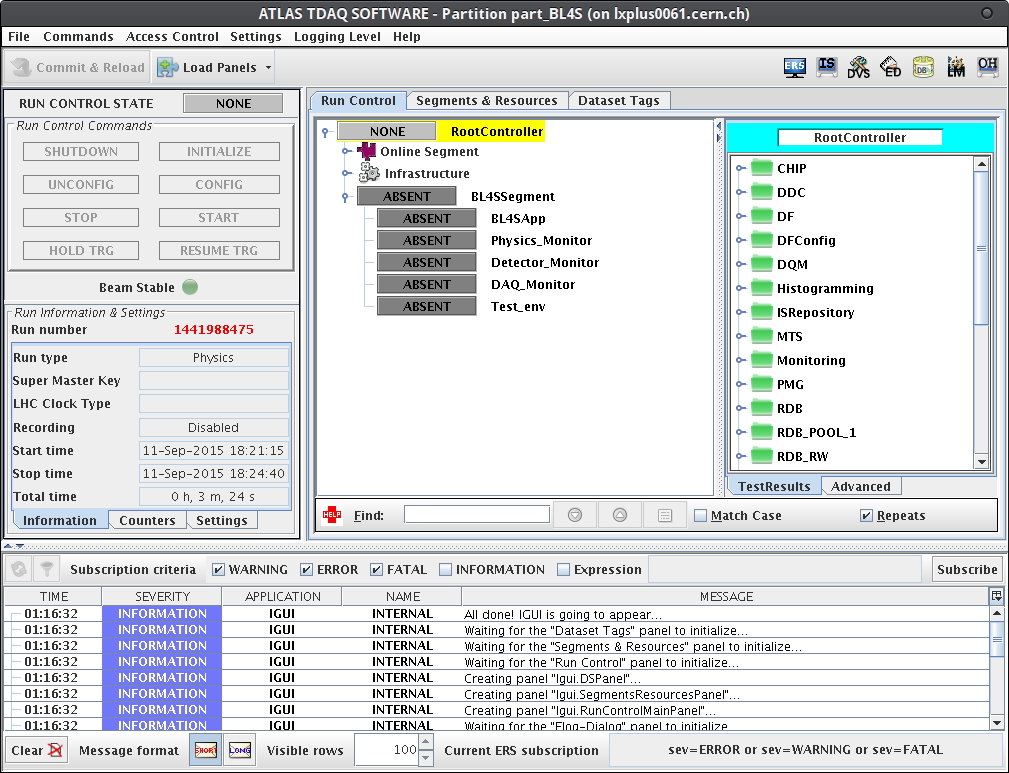
\includegraphics[scale=0.24]{img/DAQ_absent}\vspace*{-0.2cm}\caption{ATLAS DAQ software}\end{figure}\vspace*{-1cm}
\end{frame}

\begin{frame}{Data Acquisition software}
\vspace*{-1cm}
\begin{figure}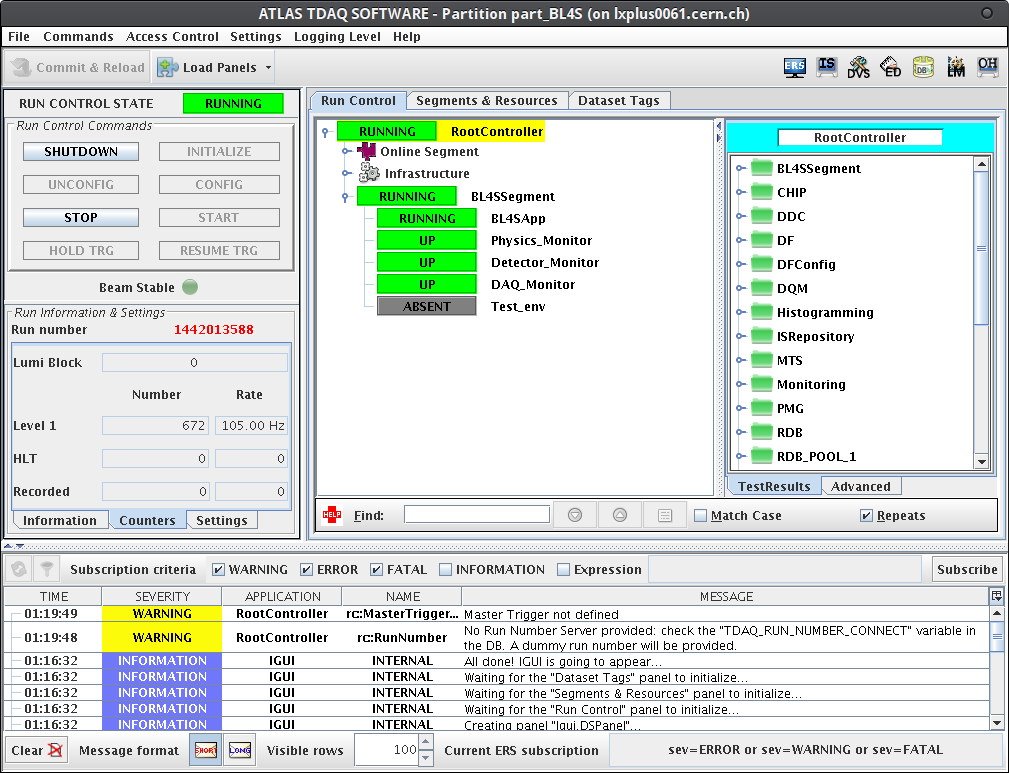
\includegraphics[scale=0.24]{img/DAQ_running}\vspace*{-0.2cm}\caption{ATLAS DAQ software}\end{figure}\vspace*{-1cm}
\end{frame}

\begin{frame}{Monitoring software}
\vspace*{-0.5cm}
\begin{figure}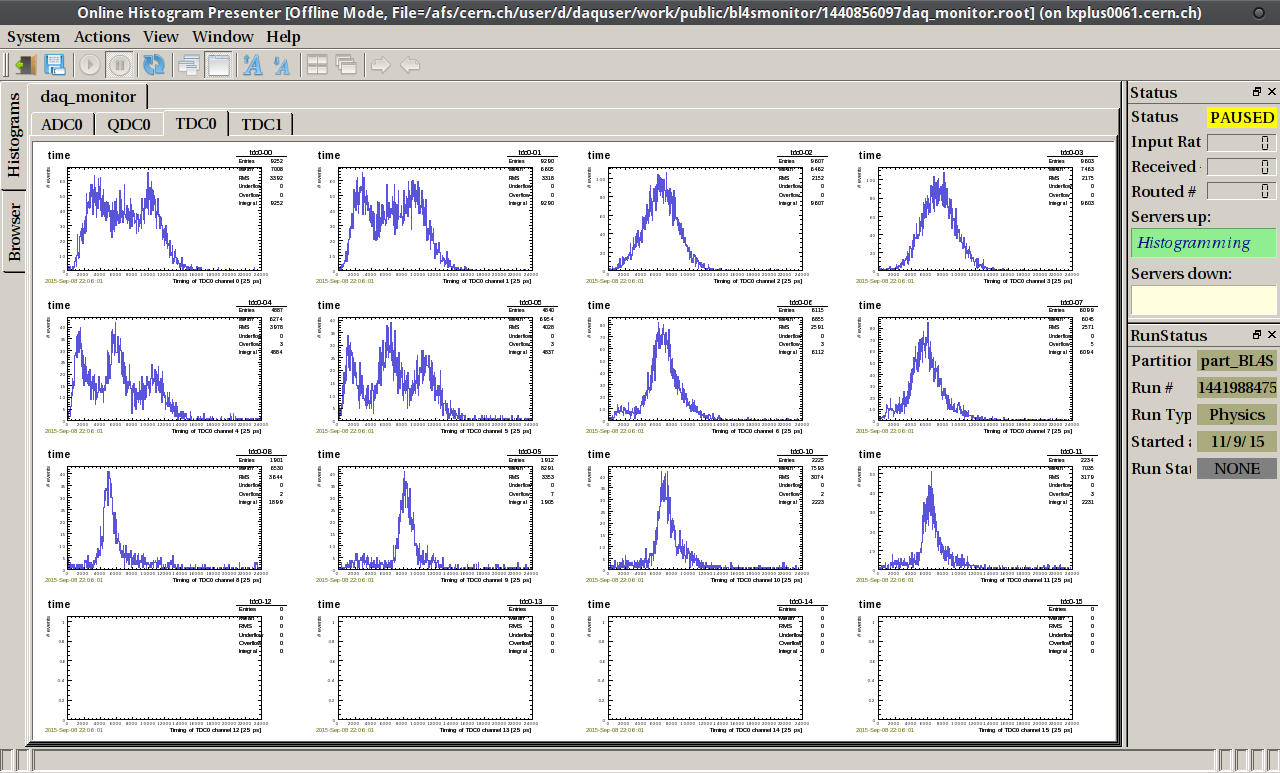
\includegraphics[scale=0.22]{img/Monitoring}\vspace*{-0.2cm}\caption{Online Histogram Presenter (OHP)}\end{figure}\vspace*{-1cm}
\end{frame}

\begin{frame}{Log book}
\vspace*{-1cm}
\begin{figure}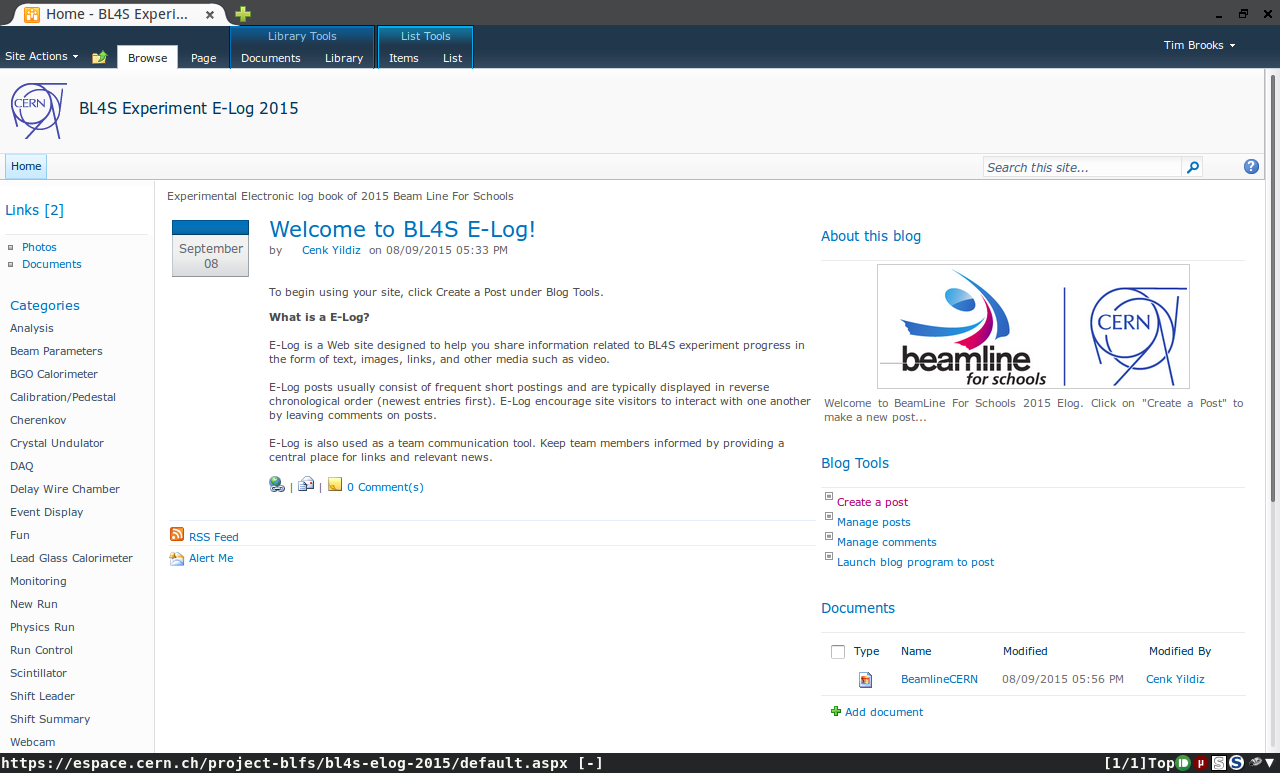
\includegraphics[scale=0.24]{img/Log_book}\vspace*{-0.2cm}\caption{BL4S online log book - it's only science if you write it down!}\end{figure}\vspace*{-1cm}
\end{frame}

\begin{frame}{Shift tasks}
\begin{enumerate}
\item Check run plan - online whiteboard
\item Check detector set-up - access:
    \begin{itemize}
        \item HV must be disabled
        \item Magnet switched off
        \item Shift leader will check the zone first
        \item All shifters can then key into the zone
    \end{itemize}
    \item Ensure HV (and LV) is on
    \item Collect calibration data - pedestal programs
    \item Check run settings before starting to record
    \item Check monitoring histograms
    \item Write a log entry when:
    \begin{itemize}
      \item Changing settings
      \item Starting/stopping a run
      \item Ending your shift
    \end{itemize}
\end{enumerate}
\end{frame}

\begin{frame}{Help}
  \begin{enumerate}
    \item Pay attention and ask questions in the morning meeting
    \item Check the log book - some problems may be known already \url{http://espace.cern.ch/project-blfs/bl4s-elog-2015/}
    \item Documentation is available on our twiki: \url{http://twiki.cern.ch/twiki/bin/view/BL4S}
    \item If you're unsure - ask your shift leader
    \item Contacts:
    \begin{itemize}
      \item Markus Joos (160663)
      \item Tim Brooks (167969)
      \item Candan Dozen (167970)
    \end{itemize}
  \end{enumerate}
\end{frame}

\end{document}
